\documentclass{article}
\usepackage[utf8]{inputenc}
\usepackage{hyperref}
\usepackage{pdfrender,xcolor}
\usepackage{graphicx}



\usepackage{amsmath,amssymb,amsthm}
\usepackage{mathtools,graphicx,tikz-cd}
\usepackage{blindtext}
\usepackage[margin = 1.25 in]{geometry}
\usepackage{enumitem}

\usepackage{fancyhdr,accents,lastpage}
\pagestyle{fancy}
\setlength{\headheight}{25pt}

\newtheorem{theorem}{Theorem}[section]
\newtheorem{corollary}{Corollary}[theorem]
\newtheorem{lemma}[theorem]{Lemma}

\theoremstyle{definition}
\newtheorem{definition}{Definition}[section]

\theoremstyle{remark}
\newtheorem*{remark}{Remark}
\newtheorem{exercise}{Exercise}
\newtheorem{example}{Example}[definition]


\DeclareMathOperator{\ab}{ab}
\DeclareMathOperator{\Aut}{Aut}
\DeclareMathOperator{\BGL}{BGL}
\DeclareMathOperator{\Br}{Br}
\DeclareMathOperator{\card}{card}
\DeclareMathOperator{\ch}{ch}
\DeclareMathOperator{\Char}{char}
\DeclareMathOperator{\CHur}{CHur}
\DeclareMathOperator{\Cl}{Cl}
\DeclareMathOperator{\coker}{coker}
\DeclareMathOperator{\Conf}{Conf}
\DeclareMathOperator{\disc}{disc}
\DeclareMathOperator{\End}{End}
\DeclareMathOperator{\et}{\text{\'et}}
\DeclareMathOperator{\Fix}{Fix}
\DeclareMathOperator{\Gal}{Gal}
\DeclareMathOperator{\GL}{GL}
\DeclareMathOperator{\Hom}{Hom}
\DeclareMathOperator{\Hur}{Hur}
\DeclareMathOperator{\im}{im}
\DeclareMathOperator{\Ind}{Ind}
\DeclareMathOperator{\Inn}{Inn}
\DeclareMathOperator{\Irr}{Irr}
\DeclareMathOperator{\lcm}{lcm}
\DeclareMathOperator{\Mor}{Mor}
\DeclareMathOperator{\ord}{ord}
\DeclareMathOperator{\Out}{Out}
\DeclareMathOperator{\Perm}{Perm}
\DeclareMathOperator{\PGL}{PGL}
\DeclareMathOperator{\Pin}{Pin}
\DeclareMathOperator{\PSL}{PSL}
\DeclareMathOperator{\rad}{rad}
\DeclareMathOperator{\sgn}{sgn}
\DeclareMathOperator{\SL}{SL}
\DeclareMathOperator{\SO}{SO}
\DeclareMathOperator{\Sp}{Sp}
\DeclareMathOperator{\Spec}{Spec}
\DeclareMathOperator{\Spin}{Spin}
\DeclareMathOperator{\St}{St}
\DeclareMathOperator{\Surj}{Surj}
\DeclareMathOperator{\Syl}{Syl}
\DeclareMathOperator{\tame}{tame}
\DeclareMathOperator{\Tr}{Tr}

\newcommand{\eps}{\varepsilon}
\newcommand{\QED}{\hspace{\stretch{1}} $\blacksquare$}
\renewcommand{\AA}{\mathbb{A}}
\newcommand{\CC}{\mathbb{C}}
\newcommand{\EE}{\mathbb{E}}
\newcommand{\FF}{\mathbb{F}}
\newcommand{\HH}{\mathbb{H}}
\newcommand{\NN}{\mathbb{N}}
\newcommand{\OO}{\mathbb{O}}
\newcommand{\PP}{\mathbb{P}}
\newcommand{\QQ}{\mathbb{Q}}
\newcommand{\RR}{\mathbb{R}}
\newcommand{\ZZ}{\mathbb{Z}}
\newcommand{\bfm}{\mathbf{m}}
\newcommand{\mcA}{\mathcal{A}}
\newcommand{\mcC}{\mathcal{C}}
\newcommand{\mcG}{\mathcal{G}}
\newcommand{\mcH}{\mathcal{H}}
\newcommand{\mcM}{\mathcal{M}}
\newcommand{\mcN}{\mathcal{N}}
\newcommand{\mcO}{\mathcal{O}}
\newcommand{\mcP}{\mathcal{P}}
\newcommand{\mcQ}{\mathcal{Q}}
\newcommand{\mfa}{\mathfrak{a}}
\newcommand{\mfb}{\mathfrak{b}}
\newcommand{\mfI}{\mathfrak{I}}
\newcommand{\mfM}{\mathfrak{M}}
\newcommand{\mfm}{\mathfrak{m}}
\newcommand{\mfo}{\mathfrak{o}}
\newcommand{\mfO}{\mathfrak{O}}
\newcommand{\mfP}{\mathfrak{P}}
\newcommand{\mfp}{\mathfrak{p}}
\newcommand{\mfq}{\mathfrak{q}}
\newcommand{\mfz}{\mathfrak{z}}
\newcommand{\AGL}{\mathbb{A}\GL}
\newcommand{\Qbar}{\overline{\QQ}}
\renewcommand{\qedsymbol}{$\blacksquare$}



\lhead{Introduction} 
\chead{Math Club}
\rhead{Fall 2020} 


\begin{document}

\section{Introduction}

Welcome to UCSB's Math Club! This quarter we will work on our problem solving skills in preparation for the Putnam competition. 

The Putnam is an olympiad style competition held the first Saturday of December every year. In the competition, you will be given 12 problems to be done over 6 hours, and generally they are quite challenging. If you can correctly answer 4 or more of the problems, you will generally be ranked in the top 300 in the nation! This year, the Putnam will at least be pushed back until February. It might even be done online. We'll provide more information once things are settled about the exam.

Of course, there is no obligation for you to take the Putnam! It is simply a convenient excuse for us to try our hand at solving tough problems, and sharpen our analytical thinking skills. The skills developed in Math Club will help you become a better mathematician in (in our opinion) a fun way! 

Today, we will get to know our new and returning members and solve a few problems together. Below we have put some resources for your perusal. Make sure you join the Facebook page and the Slack channel to keep up with the group. Happy problem solving!

\section{Resources}

The problems below are shamelessly ripped from the books \textit{Lateral Thinking Puzzlers} by Paul Sloane and \textit{The Art and Craft of Problem Solving} by Paul Zeitz. There are, of course, tons of other resources beyond this (aops.com, Kiran Kedlaya's website for past Putnam problems).

\section{Easy (not really)}

\begin{exercise}
Bottle $A$ contains a quart of milk and bottle $B$ contains a quart of black coffee. Pour a small amount from $B$ into $A$, mix well, and then pour back from $A$ into $B$ until both bottles again each contain a quart of liquid. What is the relationship between the fraction of the coffee in $A$ and the fraction of milk in $B$?
\end{exercise}

\begin{exercise}[Experiment]
Define $f(x)=1/(1-x)$ and denote $r$ iterations of the function $f$ by $f^r$, so \[f^r(x)=\underbrace{f(f(\cdots(f(x))\cdots))}_{r\text{ $f$'s}} \] Determine $f^{1999}(2000)$.
\end{exercise}

\begin{exercise}[Draw a picture]
Find the minimum value of $(u-v)^2+(\sqrt{2-u^2}-\frac{9}{v})^2$ for $0<u<\sqrt{2}$ and $v>0$.
\end{exercise}

\begin{exercise}[Choose effective notation]
One morning it started snowing at a heavy and constant rate. A snowplow started at 8:00 A.M. At 9:00 A.M. it had gone $2$ miles. By 10:00 A.M. it had gone $3$ miles. Assuming the snowplow removes a constant volume of snow per hour, determine the time at which it started snowing.
\end{exercise}

\section{Medium}

\begin{exercise}[Not a trick question]
There are four main towns in Lateralia. Call them $A$, $B$, $C$, and $D$. They lie at the corners of a ten-mile square. In order to improve communications between the towns, the Lateralian Department of Transport decided to build a new road linking all four towns together. Because they had very little money, it was decided that the new road system should be as short as possible and still allow access from any one town to any another. The engineers came up with the three designs shown below. Number one uses $40$ miles of road, number two uses $30$ miles of road, and number three uses $28.3$ miles of road. The designers naturally recommended plan number three because it employed the smallest road area and, therefore, cost the least. However, when they submitted their plan to the Minister of Finance, he accused them of extravagance and quickly pointed out a better design that required even less road surface. What was his superior solution?

\begin{center}
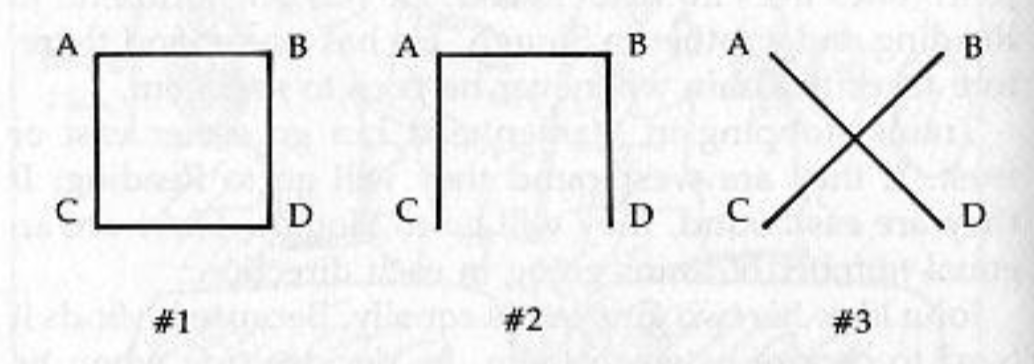
\includegraphics[scale=0.5]{pic1.png}
\end{center}
\end{exercise}

\begin{exercise}[Also not a trick question]
The governing body of the state of Lateralia was extremely concerned about the uneven distribution of wealth in the country. They thought it unfair that the richest man should have so much more than his poorer compatriots. They therefore instituted a wealth tax decreeing that each year the wealthiest man in the country had to give away his money by doubling the wealth of every other citizen, starting with the poorest and working up to the second wealthiest person if possible. The decree was carried out, and the richest person gave away his money by doubling the wealth of all other citizens. However, the governing body was shocked to find that this action had made no difference to the overall distribution of wealth nor to the relative wealth of the poorest and richest citizens. How could this be so?
\end{exercise}

\begin{exercise}[Putnam 1990]
Let $T_0=2$, $T_1=3$, $T_2=6$, and for $n\geq 3$, 
\[T_n=(n+4)T_{n-1}-4nT_{n-2}+(4n-8)T_{n-3}\] The first few terms are
\[2,3,6,14,40,152,784,5168,40576,363392 \] Find a formula for $T_n$ in the form $T_n=A_n+B_n$, where $A_n$ and $B_n$ are well-known sequences. Even better, prove that your formula works.
\end{exercise}

\section{Difficult}

\begin{exercise}
You have an equal-arm balance scale and twelve solid balls. You are told that one of the balls has a different weight from all the others, but you do not know whether it is lighter or heavier. You can weigh the balls against each other in the scale balance. Can you find the odd ball and tell if it is lighter or heavier in only three weighings?
\end{exercise}

\begin{exercise}[Putnam 1980]
Prove that there exist integers $a,b,c$, not all zero and each of absolute value less than one million, such that $|a+b\sqrt{2}+c\sqrt{3}|<10^{-11}$. Prove that if $a,b,c$ are integers that are not all zero and are each of absolute value less than one million, then $|a+b\sqrt{2}+c\sqrt{3}|>10^{-21}$.
\end{exercise}

\begin{exercise}
Let $S$ be a finite set of at least two points in the plane. Assume that no three points of $S$ are collinear. A windmill is a process that starts with a line $\ell$ going through a single point $P \in S$. The line rotates clockwise about the pivot $P$ until the first time that the line meets some other point $Q$ belonging to $S$. This point $Q$ takes over as the new pivot, and the line now rotates clockwise about $Q$, until it next meets a point of $S$. This process continues indefinitely. Show that we can choose a point $P$ in $S$ and a line $\ell$ going through $P$ such that the resulting windmill uses each point of $S$ as a pivot infinitely many times.
\end{exercise}

\end{document}